\noindent
\begin{tabular}{cc}
\begin{minipage}[l]{0.50\textwidth}
 \begin{exerciseS}[Recipiente rotante]
Un contenitore cilindrico (raggio $R$, altezza $H$) è riempito fino ad una 
 quota $h_1 =H/2$ di un liquido di densità $\rho$. Il contenitore è messo
 poi in rotazione con velocità angolare costante $\Omega$. 
Una volta esaurito il transitorio, viene chiesto di trovare:
\begin{itemize}
\item la forma che assume il liquido all’interno del contenitore;
\item la velocità $\Omega_{max}$ alla quale il liquido inizia a uscire dal contenitore;
\item il campo di pressione quando il corpo ruota con velocità angolare $\Omega_{max}$.
\end{itemize}
 \vspace{0.3cm}
(R: $z_{free}(r) = \dfrac{\Omega^2 r^2}{2 g} - \dfrac{\Omega^2 R^2}{4 g} + \dfrac{H}{2}$ \newline
 \hspace{0.5cm} $\Omega_{max} = \sqrt{\dfrac{2 g H}{R^2}} $ \newline
 \hspace{0.5cm} $P(r) = \dots$)
\end{exerciseS}
\end{minipage}
\hspace{3mm}
\begin{minipage}[r]{0.50\textwidth}
   \begin{center}
   \includegraphics[width=0.90\textwidth, trim = 0 0 0 0,clip]{./fig/vessel}
   \end{center}
\end{minipage}
\end{tabular}

\sol

\partone Soluzione esatte delle equazioni di Navier-Stokes.
 Fluido in rotazione rigida, con superficie superiore libera.

\parttwo
\begin{itemize}
\item
Si usano le equazioni di NS in coordinate cilindriche. Seguendo un procedimento
 analogo a quello svolto per ottenere la soluzione esatta di Taylor-Couette, ma senza
 trascurare l'effetto della gravità, si ottiene la seguente coppia di equazioni
\begin{equation}\label{eqn:vessel_cyl}
 \begin{cases}
  \dfrac{\partial P}{\partial z} = - \rho g \\
  \dfrac{\partial P}{\partial r} = \rho \dfrac{u_{\theta}^2}{r}
 \end{cases}
\end{equation}
Il campo di moto descrive una rotazione rigida, poichè il termine $1/r$ della soluzione
 di Taylor-Couette non è ammissibile (l'asse appartiene al dominio, non ha senso una
 velocità che tende all'infinito). La costante di proporzionalità tra $u_{\theta}$ ed $r$
 è la velocità angolare $\Omega$ per soddisfare le condizioni al controno a parete,
 $u_{\theta}(R) = \Omega R$.
\begin{equation}
  u_{\theta}(r) = \Omega r
\end{equation}
Dall'integrazione delle due equazioni (\ref{eqn:vessel_cyl}) si ottiene il campo di pressione
 $P(r,z)$, a meno di una costante di integrazione $C$
\begin{equation}\label{eqn:p}
 P(r,z) = -\rho g z + \rho \dfrac{\Omega^2 r^2}{2} + C
\end{equation}
La condizione al contorno necessaria è $P(r,z_{free}(r)) = P_a$; sulla superficie libera,
 la cui quota è descritta dalla funzione $z_{free}(r)$ (ancora incognita),
 agisce la pressione ambiente $P_a$
\begin{equation}
 P(r,z_{free}(r)) = -\rho g z_{free} + \rho \dfrac{\Omega^2 r^2}{2} + C = P_a \\
\end{equation}
\begin{equation*}
 \ \ \ \ \ \  \Downarrow
\end{equation*}
\begin{equation}\label{eqn:zfree}
 z_{free}(r) = \dfrac{\Omega^2 r^2}{2 g} - \dfrac{P_a - C}{\rho g}
\end{equation}

Per determinare la costante $C$ bisogna ricorrere alla conservazione della massa. La massa
 contenuta all'interno del recipiente non varia (fino a quando il liquido non esce). Se si 
 considera densità costante $\rho$, bisogna scrivere la conservazione del volume tra istante 
 iniziale $V_0 = \pi R^2 H/2$ e condizione a regime $V$. Il volume $V$ viene calcolato tramite
 un'integrale di volume, comodo da descrivere in coordinate cilindriche:
\begin{equation}
\begin{aligned}
 V & = \int_{\theta=0}^{2\pi} \int_{r=0}^{R} \int_{z=0}^{z=z_{free}(r)} r dr dz d\theta = \\
   & = 2 \pi \int_{r=0}^{r=R} z_free(r) r dr  = \\
   & = 2 \pi \int_{r=0}^{r=R} \dfrac{\Omega^2 r^3}{2 g} - \dfrac{P_a - C}{\rho g}r dr = \\
   & = 2 \pi \left[ \dfrac{\Omega^2 R^4}{8 g} - \dfrac{(P_a - C)}{2 \rho g} R^2  \right] = \\
   & =   \pi \left[ \dfrac{\Omega^2 R^4}{4 g} - \dfrac{(P_a - C)}{  \rho g} R^2  \right] = \\
\end{aligned}
\end{equation}
Uguagliando $V_0$ e $V$ si ottiene
\begin{equation}
  - \dfrac{(P_a - C)R}{  \rho g} = - \dfrac{\Omega^2 R^4}{4 g} + R^2 \dfrac{H}{2}
\end{equation}
termine che può essere sotituito in (\ref{eqn:zfree})
\begin{equation}\label{eqn:zfree2}
 z_{free}(r) = \dfrac{\Omega^2 r^2}{2 g} - \dfrac{\Omega^2 R^2}{4 g} + \dfrac{H}{2}
\end{equation}
La superficie libera ha la forma di un parabolide. La concavità del paraboloide è diretta
 verso l'alto e aumenta all'aumentare di $|\Omega|$ (il risultato è indipendente dal
 verso di rotazione, e quindi dal segno di $\Omega$, poichè compare con potenze pari).
 La quota del vertice $z_v = - \dfrac{\Omega^2 R^2}{4 g} +  \dfrac{H}{2}$
 invece diminuisce.
 
\item Per determinare la $\Omega_{max}$, bisogna imporre la condizione $z_{free}(r=R) = H$.
 \begin{equation}
   z_{free}(R) = \dfrac{\Omega_{max}^2 R^2}{4 g} + R^2 \dfrac{H}{2} = H 
 \Rightarrow
  \Omega_{max} = \sqrt{\dfrac{2 g H}{R^2}}
 \end{equation}


\item Per ottenere il campo di pressione, basta inserire il il valore di $C$ e $\Omega_{max}$
 nella formula (\ref{eqn:p}).



\end{itemize}
